\chapter{Session-level Packet Distribution}
\label{chap:session}

This section describes the internals of the Session-level Packet Distribution
implementation in \ns.
The section is in two parts:
the first part is an overview of 
\href{Session configuration}{Section}{sec:config},
and a ``complete'' description of the configuration parameters 
of a Session.
The second part describes the architecture, internals, and the code path
of the Session-level Packet distribution.

The procedures and functions described in this chapter can be found in
\nsf{tcl/session/session.tcl}.

Session-level Packet Distribution is oriented towards
performing multicast simulations over large topologies.
The memory requirements for some topologies using
session level simulations are:

\begin{tabular}{r @{~~~$\approx$~} r@{\,MB}}
2048 nodes, degree of connectivity = 8 & 40 \\
2049--4096 nodes & 167 \\
4097--8194 nodes & 671 \\
\end{tabular}

Note however, that session level simulations ignore qeueing delays.
Therefore, the accuracy of
simulations that use sources with a high data rate,
or those that use multiple sources that get aggregated at points
within the network is suspect.

\section{Configuration}
\label{sec:config}

Configuration of a session level simulation consists of two parts,
\href{configuration of the session level details themselves}{Section}{%
        sec:basic-config}
and 
\href{adding loss and error models to the session level abstraction
to model specific behaviours}{Section}{sec:loss-config}.

\subsection{Basic Configuration}
\label{sec:basic-config}

The basic configuration consists of creating and configuring
a  multicast session.
Each Session (\ie, a multicast tree) must be configured strictly in
this order:
(1) create and configure the session source,
(2) create the session helper and attach it to the session source, and
finally, (3) have the session members join the session.
\begin{program}
        set ns [new SessionSim]          \; preamble initialization;
        set node [$ns node]    
        set group [$ns allocaddr]

        set udp [new Agent/UDP]         \; create and configure the source;
        $udp set dst_ $group
	set src [new Application/Traffic/CBR]
	$src attach-agent $udp
        $ns attach-agent $node $udp

        $ns create-session $node $udp   \; create attach session helper to src;

        set rcvr [new Agent/NULL]        \; configure the receiver;
        $ns attach-agent $node $rcvr
        $ns at 0.0 "$node join-group $rcvr $group" \; joining the session;

        $ns at 0.1 "$src start"
\end{program}
A session level simulation scales by translating the topology
into a virtual mesh topology.
The steps involved in doing this are:
\begin{enumerate}\itemsep0pt
\item All of the classifiers and replicators are eliminated.
  Each node only stores instance variables to track its node id, and port ids.
\item Links do not consist of multiple components.
  Each link only stores instance variables to track the bandwidth and delay attributes.
\item The topology, consisting of links is translated into a virtual mesh.
\end{enumerate}
\begin{figure}
  \centerline{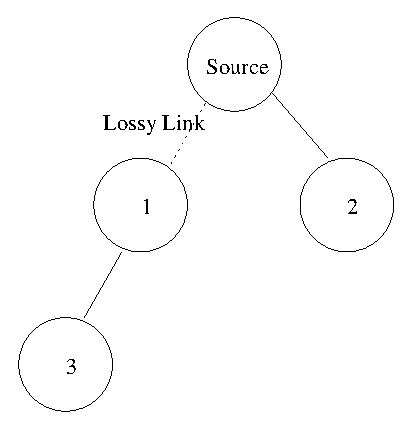
\includegraphics{regularTree}\hfil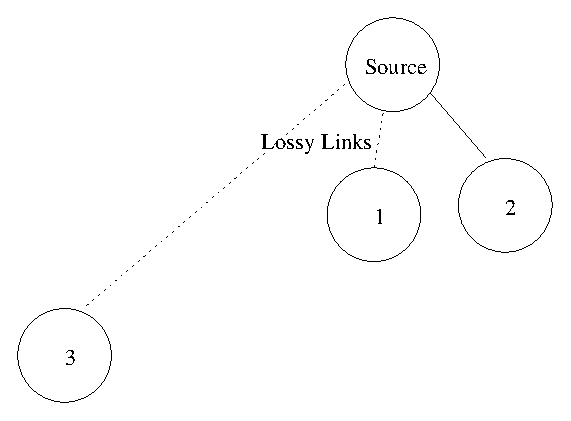
\includegraphics{sessionTree}}
  \caption{Comparison of Multicast Trees for Detailed vs. Session Routing}
  \label{fig:conversions}
\end{figure}
Figure~\ref{fig:conversions} shows the difference between a
multicast tree in a detailed simulation and one in a session level simulation.
Notice that the translation process results in a session level simulation
ignoring queuing delays.
For most simulations, \ns\ already ignores processing delays at all of the nodes.

\subsection{Inserting a Loss Module}
\label{sec:loss-config}

When studying a protocol (\eg, SRM error recovery mechanism), 
it might be useful to study protocol behavior over lossy links.
However, since a session level simulation scales by abstracting 
out the internal topology,
we need additional mechanisms to insert a loss module appropriately.
This subsection describes how one can create these loss modules to
model error scenarios.

%Please note that packets dropped at a particular link in a
%multicast tree will not be received by
%the receivers in the particular downstream subtree. We have worked 
%on this dependency problem and now the loss modules for the downstream 
%receivers will be installed automatically when a lossy link is created.

\paragraph{Creating a Loss Module}
Before we can insert a loss module in between a source-receiver pair,
we have to create the loss module.  Basically,
a loss module compares two values to decide whether to drop a packet.
The first value is obtained every time when the loss module receives 
a packet from a random variable.  The second value
is fixed and configured when the loss module is created.

The following code gives an example to create a uniform 0.1 loss rate.
\begin{program}
        # {\cf creating the uniform distribution random variable}
        set loss_random_variable [new RandomVariable/Uniform] 
        $loss_random_variable set min_ 0 \; set the range of the random variable;
        $loss_random_variable set max_ 100

        set loss_module [new ErrorModel] \; create the error model;
        $loss_module drop-target [new Agent/Null] 
        $loss_module set rate_ 10 \; set error rate to \(0.1 = 10 / (100 - 0)\);
        $loss_module ranvar $loss_random_variable \; attach random var. to loss module;
\end{program}
\href{A catalogue of the random variable distributions was described earlier}{%
        Chapter}{chap:math}.
\href{A more detailed discussion of error models was also described earlier
in a different chapter}{Chapter}{chap:error_model}.

\paragraph{Inserting a Loss Module}
A loss module can only be inserted after the corresponding receiver
has joined the group.  The example code below illustrates how
a simulation script can introduce a loss module.
\begin{program}
        set sessionhelper [$ns create-session $node $src] \; keep a handle to the loss module;
        $ns at 0.1 "$sessionhelper insert-depended-loss $loss_module $rcvr" 
\end{program}

\section{Architecture}
\label{sec:session-arch}
The purpose of Session-level packet distribution is to
speed up simulations and reduce memory consumption while 
maintaining reasonable accuracy.
The first bottleneck observed is the memory consumption by heavy-weight
links and nodes.  Therefore, in SessionSim (Simulator for Session-level
packet distribution), we keep only minimal amount of 
states for links and nodes, and connect the higher level source and 
receiver applications with appropriate delay and loss modules.
A particular source in a group sends its data packets
to a replicator that is responsible for replicating the packets
for all the receivers.
Intermediate loss and delay modules between this replicator and the receivers
will guarantee the appropriate end-to-end characteristics.
To put it another way, a session level simulation
abstracts out the topology, routing and queueing delays.
Packets in SessionSim do not get routed.  
They only follow the established Session.

\section{Internals}
This section describes the internals of Session-level Packet Distribution.
We first describe the OTcl primitives to configure a session level
simulation (Section~\ref{sec:session-objlink});
we conclude with a brief note on hos packet forwarding is achieved
(Section~\ref{sec:session-pktforward}).

\subsection{Object Linkage}
\label{sec:session-objlink}

We describe three aspects of constructing a session level simulation in
\ns:
the modified topology routines that permit the creation of abstract
nodes and links,
establish the session helper for each active source,
add receivers to the session by inserting the appropriate loss and delay
models when that receiver joins the appropriate group.

\paragraph{Nodes and Links}
The node contains only its node id and the port number for the next agent.
A link only contains the values of its bandwidth and delay.

\begin{program}
SessionNode instproc init \{\} \{
    $self instvar id_ np_
    set id_ [Node getid]
    set np_ 0
\}

SessionSim instproc simplex-link \{ n1 n2 bw delay type \} \{
    $self instvar bw_ delay_
    set sid [$n1 id]
    set did [$n2 id]

    set bw_($sid:$did) [expr [string trimright $bw Mb] * 1000000]
    set delay_($sid:$did) [expr [string trimright $delay ms] * 0.001]
\}
\end{program}

\paragraph{Session Helper}
Each active source in a session requires a ``session helper''.
The session helper in \ns\ is realised through a replicator.
This session helper is created when the user issues a
\proc[]{create-session} to identify the source agent.
The simulator itself keeps a reference to the session helper
in its instance variable array, \code{session_},
indexed by the source and destination address of the source.

Note that the destination of source agent must be set before
calling \proc[]{create-session}.

\begin{program}
SessionSim instproc create-session \{ node agent \} \{
    $self instvar session_

    set nid [$node id]
    set dst [$agent set dst_]
    set session_($nid:$dst) [new Classifier/Replicator/Demuxer]
    $agent target $session_($nid:$dst) \; attach the replicator to the source;
    return $session_($nid:$dst) \; keep the replicator in the SessionSim instance variable array \code{session_};
\}
\end{program}

\paragraph{Delay and Loss Modules}

Each receiver in a group requires a delay module that
reflects its delay with respect to the particular source.
When the receiver joins a group, 
\proc[]{join-group} identifies all session helpers in \code{session_}.
If the destination index matches the group address
the receiver are joining, then the following actions are performed.
\begin{enumerate}
\item A new slot of the session helper is created and assigned to the receiver.
\item The routine computes the accumulated bandwidth and delay
  between the source and receiver using the SessionSim instance procedures
  \proc[]{get-bw} and \proc[]{get-delay}.
\item A constant random variable is created; it will generate random delivery
  times using the accumulative delay as an estimate of the average delay.
\item A new delay module is created with the end-to-end bandwidth
  characteristics, and the random variable generator provides the delay
  estimates.
\item The delay module in inserted into the session helper and interposed
  between the helper and the receiver.
\end{enumerate}
See Section~\ref{sec:loss-config} for similarly
inserting a loss module for a receiver.

\begin{program}
SessionSim instproc join-group \{ agent group \} \{
    $self instvar session_

    foreach index [array names session_] \{
        set pair [split $index :]
        if \{[lindex $pair 1] == $group\} \{
            # Note: must insert the chain of loss, delay, 
            # and destination agent in this order:

            $session_($index) insert $agent \; insert destination agent into session replicator;

            set src [lindex $pair 0] \; find accum. b/w and delay;
            set dst [[$agent set node_] id]
            set accu_bw [$self get-bw $dst $src]
            set delay [$self get-delay $dst $src]

            set random_variable [new RandomVariable/Constant] \; set delay variable ;
            $random_variable set avg_ $delay

            set delay_module [new DelayModel] \; configure the delay module;
            $delay_module bandwidth $accu_bw
            $delay_module ranvar $random_variable

            $session_($index) insert-module $delay_module $agent \; insert the delay module;
        \}
    \}
\}
\end{program}


\subsection{Packet Forwarding}
\label{sec:session-pktforward}
Packet forwarding activities are executed in C++.  A source application 
generates a packet and forwards to its target which must be a replicator 
(session helper).  The replicator copies the packet and forwards 
to targets in the active slots which are either delay modules or loss modules. If loss modules, a decision is made whether to drop the packet.
If yes, the packet is forwarded to the loss modules drop target.  If not,
the loss module forwards it to its target which must be a delay module.
The delay module will forward the packet with a delay to its target which
must be a receiver application.
\begin{figure}[tb]
%  \centerline{\includegraphics{sessionArch}}
  \caption{Architectural Realization of a Session Level Simulation Session}
  \label{fig:session}
\end{figure}


\section{Commands at a glance}
\label{sec:sessioncommand}

Following is a list of session-level related commands:
\begin{flushleft}
\code{set ns [new SessionSim]}\\
This command creates an instance of the sessionmode simulator.


\code{$ns_ create-session <node> <agent>}\\
This command creates and attaches a session-helper, which is basically a
replicator, for the source <agent> created at the <node>.

\end{flushleft} 

\endinput

### Local Variables:
### mode: latex
### comment-column: 60
### backup-by-copying-when-linked: t
### file-precious-flag: nil
### End:
